\documentclass[preprint,12pt,a4paper]{elsarticle}
\usepackage{lmodern}
\usepackage{amssymb}
\usepackage{booktabs}
\usepackage{hyperref}
\usepackage{graphicx}
\usepackage{xcolor}
\usepackage{tikz}
\usetikzlibrary{arrows.meta,positioning,fit,shapes.geometric}
\setlength{\parindent}{0pt}
\setlength{\emergencystretch}{2em}
\journal{SoftwareX}

% Generated by the release pipeline. The fallbacks keep draft builds readable,
% while check_softwarex_release.py rejects them for publication.
\IfFileExists{generated/release_metadata.tex}{\newcommand{\ReleaseVersion}{v1.0.2}
\newcommand{\ReleaseDOI}{10.5281/zenodo.21846125}
\newcommand{\ReleaseCommit}{7a7dae6c7fd4}
\newcommand{\ReleaseDate}{2026-08-08}
}{
  \newcommand{\ReleaseVersion}{v1.0.0 release candidate}
  \newcommand{\ReleaseDOI}{release gate pending}
  \newcommand{\ReleaseCommit}{release gate pending}
  \newcommand{\ReleaseDate}{release gate pending}
}

\begin{document}
\begin{frontmatter}

\title{Medora: An open-source bilingual platform for consent-aware health-record management and appointment coordination}

\author{Sarwad Hasan Siddiqui}
\author{Adiba Tahsin}
\author{Kazi Saeed Alam\corref{cor1}}
\ead{saeed.alam@cse.kuet.ac.bd}
\cortext[cor1]{Corresponding author.}
\address{Department of Computer Science and Engineering, Khulna University of Engineering \& Technology, Khulna 9203, Bangladesh}

\begin{abstract}
Health records, paper prescriptions, and appointment workflows are often split
across unrelated systems. The cost of that fragmentation is especially visible in
bilingual, mobile-first settings, where a patient may carry the only copy of a
handwritten prescription. Medora is open-source research software that combines
patient-managed records, appointment coordination, human-reviewed prescription
digitization, and specialty navigation in English and Bangla. The implementation
separates local processing from three external
data paths: document images, text generation, and live audio. Each external path
requires a purpose-specific, revocable consent grant. OCR and generated summaries
remain review-required drafts, while appointment uniqueness is enforced in the
database and delivery events are published through a transactional outbox. The
release includes a public prescription corpus, an assisted annotation tool, frozen
evaluation configurations, safety fixtures, and raw reproducibility artifacts.
Medora has not been clinically validated and is not presented as a medical device
or a production-ready clinical system.
\end{abstract}

\begin{keyword}
digital health \sep bilingual software \sep consent \sep prescription OCR \sep appointment coordination \sep reproducibility
\end{keyword}
\end{frontmatter}

\section*{Code metadata}
\begin{table}[!h]
\small
\begin{tabular}{@{}p{0.05\textwidth}p{0.35\textwidth}p{0.53\textwidth}@{}}
\toprule
& Description & Value \\
\midrule
C1 & Current code version & \ReleaseVersion \\
C2 & Permanent archive & \ReleaseDOI \\
C3 & Repository & \url{https://github.com/CSE-3200-System-Project/Medora}; tested commit \ReleaseCommit \\
C4 & Legal code license & MIT License \\
C5 & Version control & Git \\
C6 & Languages and services & Python, TypeScript, SQL; FastAPI, Next.js, PostgreSQL; optional PaddleOCR, Azure Document Intelligence, hosted text models, faster-whisper, and Vapi \\
C7 & Environment & Python 3.11, Node.js 20, PostgreSQL 15, or the checksummed release containers \\
C8 & Documentation & \url{https://github.com/CSE-3200-System-Project/Medora/tree/main/docs} \\
C9 & Support & saeed.alam@cse.kuet.ac.bd \\
\bottomrule
\end{tabular}
\caption{Code metadata. The archived release date is \ReleaseDate.}
\end{table}

\section{Motivation and significance}

Medora addresses a practical research problem: how can a bilingual web platform
connect records, paper documents, and appointment workflows without allowing its
assistive features to become unreviewed clinical authority? The intended users of
the software artifact are health-informatics researchers, software-engineering
educators, and teams studying consent, handwriting recognition, or concurrency in
resource-constrained settings. It is not a substitute for an institutional
electronic medical record or professional medical judgment.

Established open-source systems cover a wider institutional scope. OpenMRS offers a
modular medical-record platform and service layer; Bahmni combines OpenMRS with
laboratory, imaging, and enterprise-resource components for low-resource hospitals;
GNU Health provides hospital, laboratory, public-health, localization, and Fast
Healthcare Interoperability Resources (FHIR) modules~\cite{openmrs,bahmni,gnuhealth}.
Medora instead supplies a smaller mobile-oriented research implementation linking
patient-held records and booking with consent-aware experiments. These projects are
complements rather than direct performance baselines.

Document OCR research has combined recognition, layout detection, and domain
post-processing for prescriptions and other difficult handwriting~\cite{du2020,
prescriptionocr}. Clinical summarization work likewise shows that fluency is not
enough: faithfulness and traceability must be evaluated separately~\cite{shing2021,
tracsum}. Symptom-checker studies report wide variation in diagnostic and urgency
recommendations~\cite{wallace2022}. Medora therefore avoids diagnosis and triage.
It offers specialty candidates for navigation, preserves manual browsing, and runs
deterministic emergency red-flag rules before any model request.

The implementation includes purpose-specific external-processing consent,
review-gated OCR, source-linked summaries, transactionally idempotent booking with
post-commit delivery, and a reproducible bilingual evaluation package. These
boundaries can be inspected in working software. They are not evidence of clinical
effectiveness.

\section{Software description}

\subsection{Architecture and trust boundaries}

Medora consists of a Next.js web client, a FastAPI core API, a separate FastAPI OCR
service, and PostgreSQL (Fig.~\ref{fig:trust}). Authentication identifies the actor;
backend role, ownership, care-relationship, appointment-state, and consent checks
then authorize each operation. Frontend visibility is only a usability aid. The
published permission matrix states these predicates for patients, doctors, and
administrators.

\begin{figure}[!h]
\centering\resizebox{\textwidth}{!}{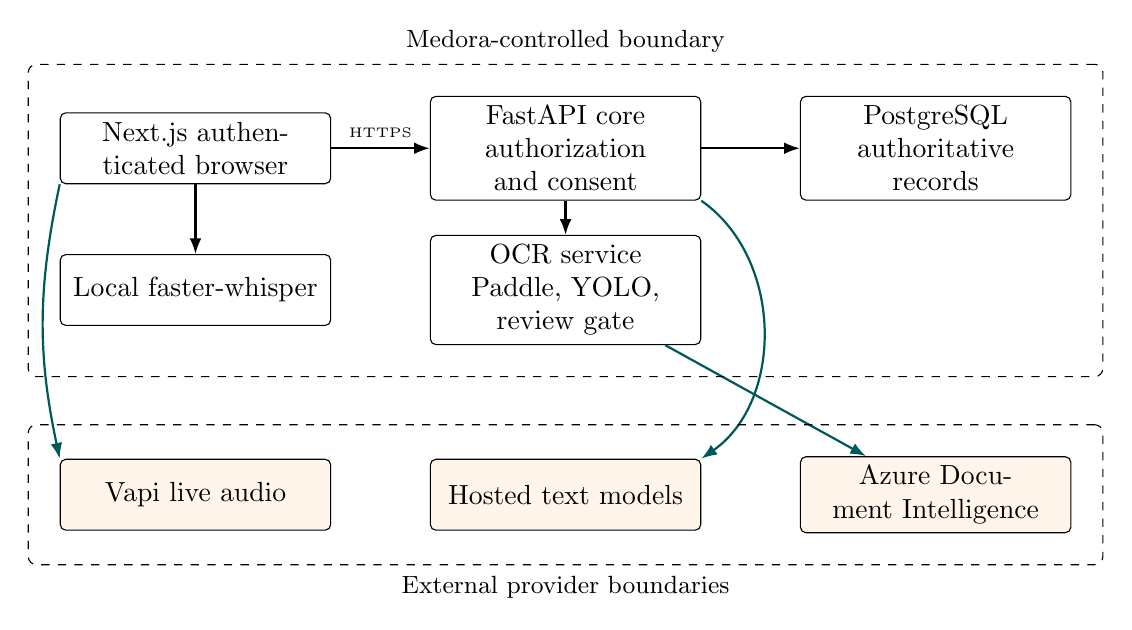
\begin{tikzpicture}[
  box/.style={draw, rounded corners=2pt, align=center, minimum height=9mm, text width=32mm, fill=white},
  boundary/.style={draw, dashed, rounded corners=3pt, inner sep=4mm},
  flow/.style={-{Latex[length=2mm]}, thick},
  consent/.style={-{Latex[length=2mm]}, thick, teal!70!black},
  external/.style={draw, rounded corners=2pt, align=center, minimum height=9mm, text width=32mm, fill=orange!8},
  grant/.style={font=\scriptsize, fill=white, inner sep=1.5pt, text=teal!70!black}
]
\node[box] (browser) at (0,0) {Next.js authenticated browser};
\node[box] (backend) at (4.7,0) {FastAPI core\\authorization and consent};
\node[box] (db) at (9.4,0) {PostgreSQL\\authoritative records};
\node[box] (whisper) at (0,-1.8) {Local faster-whisper};
\node[box] (ocr) at (4.7,-1.8) {OCR service\\Paddle, YOLO, review gate};

\node[external] (vapi) at (0,-4.4) {Vapi live audio};
\node[external] (llm) at (4.7,-4.4) {Hosted text models};
\node[external] (azure) at (9.4,-4.4) {Azure Document Intelligence};

\draw[flow] (browser) -- node[above, font=\tiny]{HTTPS} (backend);
\draw[flow] (backend) -- (db);
\draw[flow] (backend) -- (ocr);
\draw[flow] (browser) -- (whisper);
\draw[consent] (browser.south west) to[bend right=12] (vapi.north west);
\draw[consent] (backend.south east) to[out=-35,in=35] (llm.north east);
\draw[consent] (ocr) -- (azure);

\node[boundary, fit=(browser)(backend)(db)(ocr)(whisper)] (medora-boundary) {};
\node[font=\small, fill=white, inner sep=1pt, anchor=south]
  at ([yshift=1mm]medora-boundary.north) {Medora-controlled boundary};
\node[boundary, fit=(vapi)(llm)(azure)] (provider-boundary) {};
\node[font=\small, fill=white, inner sep=1pt, anchor=north]
  at ([yshift=-1mm]provider-boundary.south) {External provider boundaries};
\end{tikzpicture}
}
\caption{Deployment and trust boundaries. Local OCR and speech recognition do not
cross an external-processing boundary. Azure document OCR, hosted text models, and
Vapi live audio are distinct recipients with separate grants.}
\label{fig:trust}
\end{figure}

Processing is deny-by-default (Fig.~\ref{fig:consent}). A grant records subject,
recipient/provider, purpose, scopes, policy version, validity, grant and revocation
times, and audit metadata. Missing, expired, revoked, or wrong-scope grants produce a
typed denial and offer a local path where one exists. Revocation blocks later
processing but cannot retract prior disclosure. Local mode never falls back to a
cloud service. When layout detection is reliable, the OCR service crops the
prescription region locally before Azure receives it.

\begin{figure}[!h]
\centering\resizebox{\textwidth}{!}{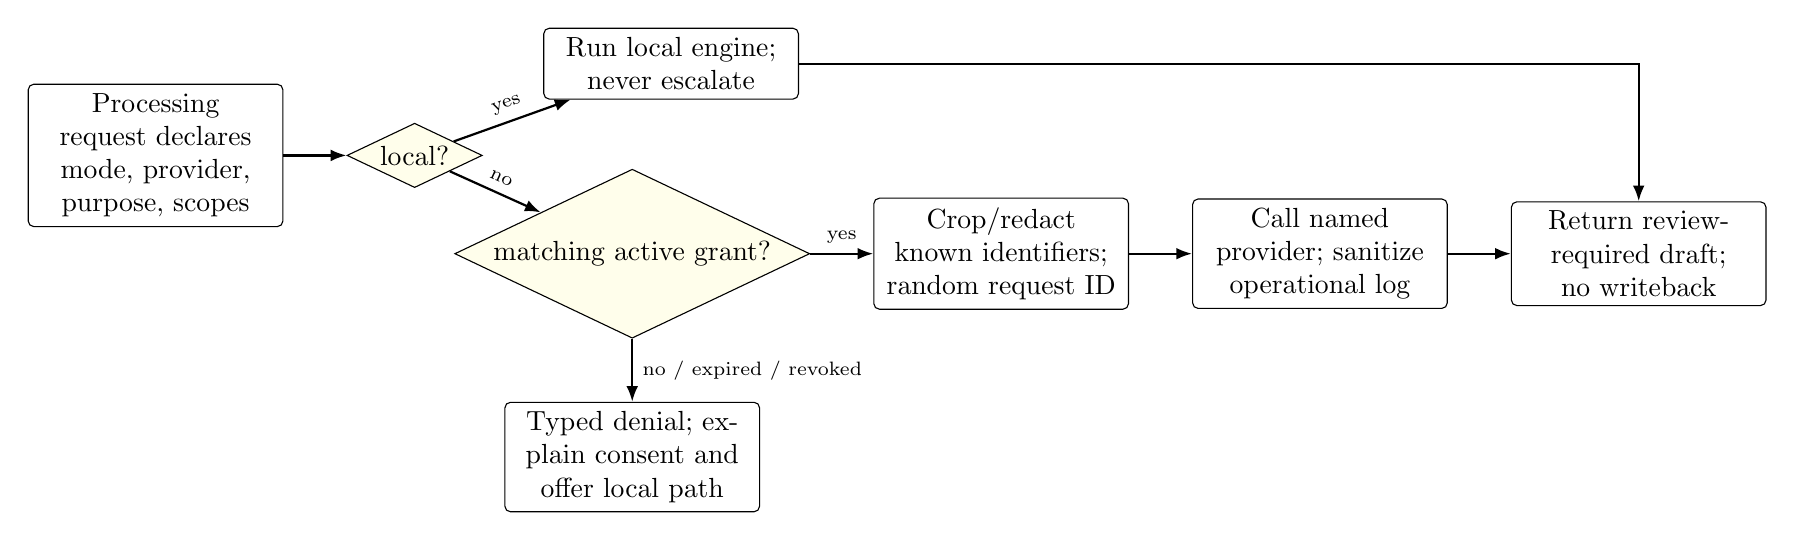
\begin{tikzpicture}[
  node distance=8mm and 8mm,
  flowbox/.style={draw, rounded corners=2pt, align=center, minimum height=9mm, text width=30mm, fill=white},
  decision/.style={draw, diamond, aspect=2.1, align=center, inner sep=1.5pt, fill=yellow!8},
  flow/.style={-{Latex[length=2mm]}, thick}
]
\node[flowbox] (request) {Processing request declares mode, provider, purpose, scopes};
\node[decision, right=of request] (local) {local?};
\node[flowbox, above right=5mm and 12mm of local] (localrun) {Run local engine; never escalate};
\node[decision, below right=5mm and 12mm of local] (grant) {matching active grant?};
\node[flowbox, right=of grant] (redact) {Crop/redact known identifiers; random request ID};
\node[flowbox, right=of redact] (provider) {Call named provider; sanitize operational log};
\node[flowbox, below=of grant] (deny) {Typed denial; explain consent and offer local path};
\node[flowbox, right=of provider] (draft) {Return review-required draft; no writeback};
\draw[flow] (request) -- (local);
\draw[flow] (local) -- node[above, sloped, font=\scriptsize]{yes} (localrun);
\draw[flow] (local) -- node[above, sloped, font=\scriptsize]{no} (grant);
\draw[flow] (grant) -- node[above, font=\scriptsize]{yes} (redact);
\draw[flow] (grant) -- node[right, font=\scriptsize]{no / expired / revoked} (deny);
\draw[flow] (redact) -- (provider);
\draw[flow] (provider) -- (draft);
\draw[flow] (localrun) -| (draft);
\end{tikzpicture}
}
\caption{Consent-aware processing. The named purpose and provider are checked before
external processing; all outputs remain non-authoritative drafts.}
\label{fig:consent}
\end{figure}

Known structured fields and common bilingual patterns for email, telephone,
address, national/passport identifiers, account identifiers, and dates are redacted
before hosted text processing. Random request identifiers replace stable subject
headers. Raw text, transcripts, prompts, and findings are not logged by default.
This reduces exposure but does not make data anonymous: unknown or indirect
identifiers can remain, and provider retention is governed by the provider terms
recorded for each execution.

\subsection{Reviewable clinical semantics}

Prescription OCR returns an unconfirmed draft with processing mode, provider,
confidence, warnings, and \texttt{authoritative\_writeback=false}. A person must correct and
verify every row before it can affect medication records. A patient's later action
is called \texttt{receipt\_acknowledged} or \texttt{discrepancy\_reported}; neither means that a
medicine is appropriate. Deprecated accept/reject routes retain compatibility for
one release but map to those meanings.

Generated summaries are read-only. Every item includes its source type, record
identifier, timestamp, and conflict or missing-evidence state. The interface keeps a
clinician-verification warning visible and provides no automatic writeback.
Specialty search returns candidates, explanations, uncertainty, and manual browse
controls. Deterministic red flags replace model output with emergency-care guidance
and do not rank specialists.

The service worker caches only versioned static assets and explicitly public
resources. Health-data writes are not background-synchronized. Logout clears Medora
caches, IndexedDB, session storage, and sensitive local storage.

\subsection{Appointment transaction and delivery}

Creating an appointment requires an \texttt{Idempotency-Key}. The backend locks the key and
slot, validates availability, and writes the appointment, idempotency result, audit
record, and outbox event in one transaction. A uniqueness constraint remains the
last defense against active duplicate slots. Only committed outbox events are
published (Fig.~\ref{fig:booking}). Realtime messages improve responsiveness; after
reconnect, clients query PostgreSQL because it remains authoritative.

\begin{figure}[!h]
\centering\resizebox{\textwidth}{!}{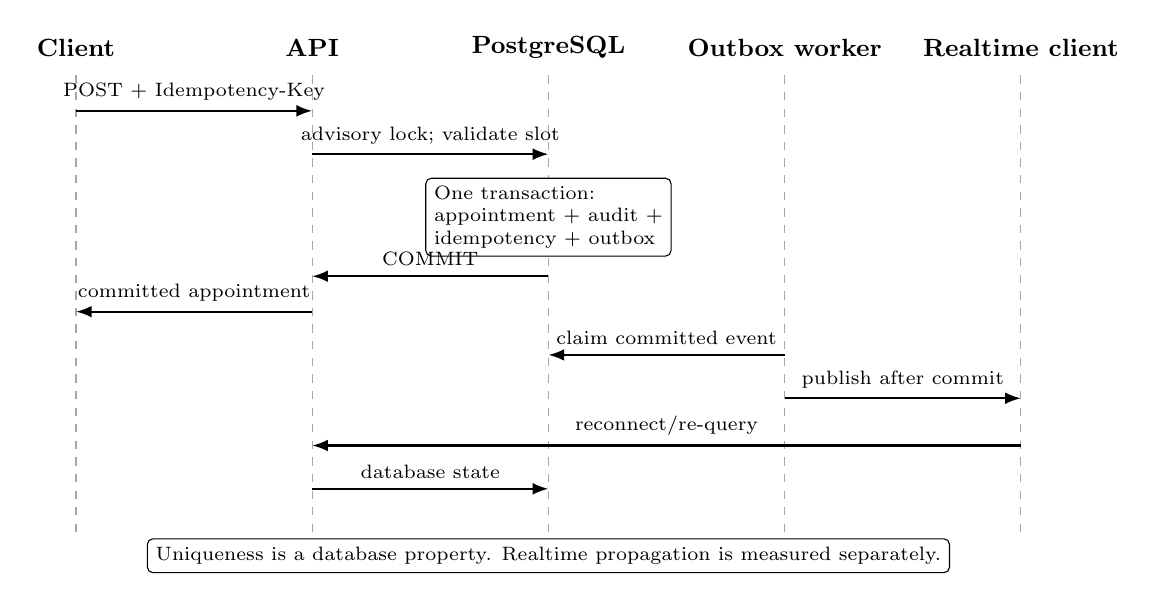
\begin{tikzpicture}[
  lifeline/.style={gray!70, dashed},
  msg/.style={-{Latex[length=2mm]}, thick},
  note/.style={draw, rounded corners=2pt, fill=white, align=left, font=\scriptsize, inner sep=3pt}
]
\foreach \x/\name in {0/Client,3/API,6/PostgreSQL,9/Outbox worker,12/Realtime client}{
  \node[font=\small\bfseries] at (\x,0) {\name};
  \draw[lifeline] (\x,-0.35) -- (\x,-6.2);
}
\draw[msg] (0,-0.8) -- node[above,font=\scriptsize]{POST + Idempotency-Key} (3,-0.8);
\draw[msg] (3,-1.35) -- node[above,font=\scriptsize]{advisory lock; validate slot} (6,-1.35);
\node[note] at (6,-2.15) {One transaction:\\appointment + audit +\\idempotency + outbox};
\draw[msg] (6,-2.9) -- node[above,font=\scriptsize]{COMMIT} (3,-2.9);
\draw[msg] (3,-3.35) -- node[above,font=\scriptsize]{committed appointment} (0,-3.35);
\draw[msg] (9,-3.9) -- node[above,font=\scriptsize]{claim committed event} (6,-3.9);
\draw[msg] (9,-4.45) -- node[above,font=\scriptsize]{publish after commit} (12,-4.45);
\draw[msg] (12,-5.05) -- node[above,font=\scriptsize]{reconnect/re-query} (3,-5.05);
\draw[msg] (3,-5.6) -- node[above,font=\scriptsize]{database state} (6,-5.6);
\node[note] at (6,-6.45) {Uniqueness is a database property. Realtime propagation is measured separately.};
\end{tikzpicture}

}
\caption{Booking timeline. Transaction consistency ends at commit; notification and
realtime propagation are later events and are measured separately.}
\label{fig:booking}
\end{figure}

\section{Evaluation and reproducibility}

The release keeps all 105 public prescription images. SHA-256 inventory identifies
two duplicate files, so metrics use 103 unique prescriptions. Reviewer-confirmed
writer/template groups are split deterministically into 21 development and 82 held-
out test records, stratified by difficulty and language. Hashes are frozen before
tuning; the test set is evaluated once.

PaddleOCR, Azure full-image OCR, and the current pipeline create assisted drafts.
A trained author corrects every record. A licensed clinician or pharmacist then
labels all unique records independently in a clean, blinded workspace. An
adjudicator resolves disagreements. Only adjudicated labels become gold data, and
pre-adjudication text and field agreement are reported. Model output is never called
ground truth.

Eight fixed configurations isolate Paddle full-image OCR (A), Azure full-image OCR
(B), YOLO region detection (C), exact catalog matching (D), fuzzy matching (E),
dosage/frequency/duration/quantity grammar (F), Bangla normalization (G), and
confidence validation with review gating (H). Immutable response caches ensure that
downstream stages consume the same OCR text. The scorer reports Rx-region character
and word error rates; per-field precision, recall, and F1; complete-row and complete-
prescription exact match; false catalog corrections; review rate and coverage; and
provider versus local runtime. Confidence intervals use paired prescription-level
bootstrap resampling. Denominators, provider failures, exclusions, configurations,
and raw scores are published.

\IfFileExists{generated/ocr_results.tex}{\input{generated/ocr_results.tex}}{
\textit{OCR results are intentionally absent from this release-candidate draft. The
release gate requires independently reviewed labels and a generated table.}}

The privacy suite contains 130 synthetic bilingual cases spanning known identifier
classes, over-redaction, consent state, prompt injection, and unknown-identifier
limitations. Separate clinician-reviewed navigation fixtures cover emergency flags,
uncertainty, correction, and manual bypass. Summary fixtures cover allergy, dose,
negation, time, duplication, conflict, missing evidence, malformed output, and
provider failure. Deterministic mock-provider and live-provider results are never
pooled.

Booking contention is run at 2, 10, and 50 concurrent attempts for 30 fresh-slot
repetitions per level after warm-up. The harness requires one committed appointment,
no duplicate row, stable idempotent replay, rollback-safe retry, and post-commit
outbox processing. Transaction latency and propagation latency are separate outputs.

\IfFileExists{generated/booking_results.tex}{\begin{table}[!h]
\centering\small
\resizebox{\linewidth}{!}{%
\begin{tabular}{@{}rrrrr@{}}
\toprule
Concurrency & Passed / 30 & Transaction p95 (ms) & Outbox p95 (ms) & Unique commit \\
\midrule
2 & 30 / 30 & 38.8 & 67.7 & yes \\
10 & 30 / 30 & 580.8 & 696.0 & yes \\
50 & 30 / 30 & 1571.5 & 1520.9 & yes \\
\bottomrule
\end{tabular}%
}
\caption{Booking contention. Transaction and post-commit outbox propagation latency are distinct measurements.}
\label{tab:booking-results}
\end{table}
}{}
\IfFileExists{generated/safety_results.tex}{\begin{table}[!h]
\centering\small
\begin{tabular}{@{}lrrl@{}}
\toprule
Suite & Cases & No undisclosed failure & Review state \\
\midrule
Bilingual privacy & 134 & 134 & synthetic \\
Symptom navigation & 30 & 30 & required \\
Source-grounded summaries & 12 & 12 & fixtures \\
\bottomrule
\end{tabular}
\caption{Safety fixture results. A case passes when it exposes no \emph{undisclosed} failure; measured detection rates are reported separately in Table~\ref{tab:privacy-span-results}. Clinician review state is reported explicitly.}
\label{tab:safety-results}
\end{table}
\begin{table}[!h]
\centering\small
\begin{tabular}{@{}lrrrr@{}}
\toprule
Expected class & Cases & Recorded & Mock & Documented \\
\midrule
emergency & 5 & 5 & 5 & 0 \\
manual\_browse & 2 & 0 & 0 & 2 \\
specialty\_candidates & 18 & 10 & 6 & 7 \\
uncertain & 5 & 2 & 2 & 0 \\
\midrule
Emergency false positives & 5 & -- & -- & -- \\
Emergency false negatives & 0 & -- & -- & -- \\
\bottomrule
\end{tabular}
\caption{Symptom-navigation fixtures. \emph{Recorded} and \emph{Mock} count agreement with the labelled class when the classifier is driven by a recorded provider intent and by the deterministic mock provider respectively; they are measurements, not pass/fail. \emph{Documented} counts cases carrying a written limitation. Emergency false positives are keyword matches on negated, third-person, or historical mentions.}
\label{tab:navigation-results}
\end{table}
\begin{table*}[!ht]
\centering\scriptsize
\begin{tabular}{@{}lrrrrr@{}}
\toprule
Identifier group & Cases & Precision & Recall & False redaction & Documented limitations \\
\midrule
account\_id & 7 & 100.0\% & 71.4\% & 0.0\% & 3 \\
address & 7 & 100.0\% & 71.4\% & 0.0\% & 2 \\
benign & 21 & -- & -- & 14.3\% & 3 \\
clinician & 4 & 100.0\% & 20.0\% & 0.0\% & 3 \\
consent & 10 & -- & -- & -- & 0 \\
date & 6 & 100.0\% & 50.0\% & 0.0\% & 3 \\
email & 9 & 100.0\% & 55.6\% & 0.0\% & 4 \\
injection & 10 & 100.0\% & 100.0\% & 0.0\% & 0 \\
limitation & 10 & -- & -- & 0.0\% & 10 \\
mixed\_script & 4 & 100.0\% & 100.0\% & 0.0\% & 0 \\
name\_labeled & 11 & 90.9\% & 90.9\% & 9.1\% & 3 \\
name\_unlabeled & 5 & -- & 0.0\% & 0.0\% & 5 \\
national\_id & 9 & 100.0\% & 100.0\% & 0.0\% & 5 \\
opaque\_id & 4 & 100.0\% & 100.0\% & 0.0\% & 0 \\
passport & 6 & 100.0\% & 66.7\% & 0.0\% & 2 \\
phone & 11 & 100.0\% & 100.0\% & 0.0\% & 0 \\
\midrule
All production-path cases & 134 & 94.7\% & 75.5\% & 3.2\% & 43 \\
\bottomrule
\end{tabular}
\caption{Span-level privacy metrics measured on the production call path, which supplies no known identifiers to the redactor. A dash means the group annotates no span for that denominator. Recall below 100\% reflects identifier forms the redactor does not claim to detect, chiefly unlabelled personal names, clinician details in prose, month-name dates, and obfuscated contact formats; every such case is enumerated with a written limitation in the archived results file. Undisclosed failures are zero by construction of the release gate.}
\label{tab:privacy-span-results}
\end{table*}
}{}

The provider manifest records provider, model, application programming interface
version, region, temperature, context limit, timeout, retries, fallback policy,
execution date, retention assumption, and paid-service requirement. Installation,
clean-container commands, model and image checksums, raw output, and table-generation
instructions accompany the archive.

\section{Illustrative examples}

\textit{Prescription extraction.} A synthetic image contains “Napa 500 mg,
1+0+1, 5 days.” Local OCR produces a draft and marks uncertain fields. The reviewer
compares the full image and Rx crop, corrects the medicine and schedule, and confirms
the record. Until that final action, no medication record changes. Cloud mode follows
the same review path but first requires an Azure-specific document consent grant.

\textit{Concurrent booking.} Two synthetic patients submit the same fresh slot at
the same time with different idempotency keys. The database commits one appointment;
the other request receives a conflict. Repeating the winning request with its key
returns the original appointment. A delayed realtime event cannot create another
row, and a reconnecting client reloads the committed database state.

\section{Impact and limitations}

Medora provides a compact test bed for studying bilingual OCR annotation, consent
state machines, source traceability, and transaction/event boundaries in one
system. The corpus and annotation tool can support comparisons beyond the bundled
pipeline, while the mock provider makes interface and failure tests reproducible
without paid credentials.

The limitations are substantial. The prescription corpus is small, identifiable,
and drawn from a limited setting; public authorization does not make it anonymous or
representative. Handwriting, language, image quality, and medicine catalogs will
shift elsewhere. Structured redaction misses unknown and indirect identifiers.
Emergency rules cannot cover every presentation. Generated summaries and specialty
candidates may omit or distort facts. Provider behavior, cost, region, and retention
can change. The concurrency benchmark demonstrates database behavior in its tested
environment, not universal capacity. No clinical trial, prospective deployment
study, regulatory assessment, penetration test, or independent clinical validation
has been completed. Any real deployment needs local governance, security review,
professional oversight, and validation for its population and intended use.

\section{Ethics and data availability}

Written authorization permits permanent public download of the identifiable images
and their inclusion in the Zenodo software archive. The final archive states the
authority, date, reference, and exact scope without publishing private
correspondence. Images are excluded from the blanket open-data license and carry a
separate notice prohibiting re-identification and unauthorized secondary use.
Annotations, synthetic fixtures, and aggregate results use CC BY 4.0; code uses the
MIT License. Public disclosure cannot guarantee later deletion of copies.

\section{Conclusions}

Medora is research software for bilingual records, review-gated prescription OCR,
specialty navigation, and appointment coordination. It makes authority and trust
boundaries explicit: external processing needs a matching
grant, generated clinical text remains a sourced draft, and database consistency is
not confused with event-delivery speed. The fixed release couples the implementation
to its corpus, protocol, raw evidence, commit, and archive DOI. It should be judged
as an inspectable platform for software research, not as a clinically validated or
production-ready medical system.

\section*{CRediT authorship contribution statement}
\textbf{Sarwad Hasan Siddiqui:} Conceptualization, Software, Data curation, Writing--original draft. \textbf{Adiba Tahsin:} Software, Data curation, Validation, Writing--original draft. \textbf{Kazi Saeed Alam:} Supervision, Resources, Writing--review and editing.

\section*{Declaration of competing interest}
The authors declare no known competing financial interests or personal relationships
that could have influenced this work.

\section*{Declaration of generative AI and AI-assisted technologies in writing}
An AI-assisted writing and coding tool was used during revision. The authors checked
the manuscript, code, citations, and generated evidence and accept responsibility
for the submitted work.

\begin{thebibliography}{00}
\bibitem{openmrs} OpenMRS Community, Architecture, \url{https://devmanual.openmrs.org/technology/architecture/}, accessed 2026.
\bibitem{bahmni} Bahmni Coalition, Bahmni: Open Source EMR \& Hospital Information System, \url{https://www.bahmni.org/}, accessed 2026.
\bibitem{gnuhealth} GNU Solidario, GNU Health Hospital Information System documentation, \url{https://docs.gnuhealth.org/his/}, accessed 2026.
\bibitem{du2020} Y. Du et al., PP-OCR: A practical ultra lightweight OCR system, arXiv:2009.09941 (2020).
\bibitem{prescriptionocr} S. Haque et al., Preserving medical information from doctor's prescription ensuring relation among the terminology, Expert Systems with Applications 255 (2024) 124640.
\bibitem{shing2021} H.-C. Shing et al., Towards clinical encounter summarization: Learning to compose discharge summaries from prior notes, arXiv:2104.13498 (2021).
\bibitem{tracsum} C. Bo et al., TracSum: Aspect-based summarization with sentence-level traceability in the medical domain, Proc. EMNLP (2025).
\bibitem{wallace2022} W. Wallace et al., The diagnostic and triage accuracy of digital and online symptom checker tools: a systematic review, npj Digital Medicine 5 (2022) 118.
\end{thebibliography}

\end{document}
